% THIS IS SIGPROC-SP.TEX - VERSION 3.1
% WORKS WITH V3.2SP OF ACM_PROC_ARTICLE-SP.CLS
% APRIL 2009
%
% It is an example file showing how to use the 'acm_proc_article-sp.cls' V3.2SP
% LaTeX2e document class file for Conference Proceedings submissions.
% ----------------------------------------------------------------------------------------------------------------
% This .tex file (and associated .cls V3.2SP) *DOES NOT* produce:
%       1) The Permission Statement
%       2) The Conference (location) Info information
%       3) The Copyright Line with ACM data
%       4) Page numbering
% ---------------------------------------------------------------------------------------------------------------
% It is an example which *does* use the .bib file (from which the .bbl file
% is produced).
% REMEMBER HOWEVER: After having produced the .bbl file,
% and prior to final submission,
% you need to 'insert'  your .bbl file into your source .tex file so as to provide
% ONE 'self-contained' source file.
%
% Questions regarding SIGS should be sent to
% Adrienne Griscti ---> griscti@acm.org
%
% Questions/suggestions regarding the guidelines, .tex and .cls files, etc. to
% Gerald Murray ---> murray@hq.acm.org
%
% For tracking purposes - this is V3.1SP - APRIL 2009

\documentclass{acm_proc_article-sp}

\usepackage{xcolor}
\newif\ifdraft
\drafttrue
%\draftfalse                                                                                                                                     
\ifdraft
\newcommand{\zhaonote}[1]{{\textcolor{cyan}{ ***Zhao: #1 }}}
\newcommand{\note}[1]{ {\textcolor{red}{\bf #1 }}}
\else
\newcommand{\zhaonote}[1]{}
\newcommand{\note}[1]{}
\fi

\begin{document}

\title{Design Principles for Modular and Scalable \linebreak Scientific Analysis Systems}
%
% You need the command \numberofauthors to handle the 'placement
% and alignment' of the authors beneath the title.
%
% For aesthetic reasons, we recommend 'three authors at a time'
% i.e. three 'name/affiliation blocks' be placed beneath the title.
%
% NOTE: You are NOT restricted in how many 'rows' of
% "name/affiliations" may appear. We just ask that you restrict
% the number of 'columns' to three.
%
% Because of the available 'opening page real-estate'
% we ask you to refrain from putting more than six authors
% (two rows with three columns) beneath the article title.
% More than six makes the first-page appear very cluttered indeed.
%
% Use the \alignauthor commands to handle the names
% and affiliations for an 'aesthetic maximum' of six authors.
% Add names, affiliations, addresses for
% the seventh etc. author(s) as the argument for the
% \additionalauthors command.
% These 'additional authors' will be output/set for you
% without further effort on your part as the last section in
% the body of your article BEFORE References or any Appendices.

%  in this sample file, there are a *total*
% of EIGHT authors. SIX appear on the 'first-page' (for formatting
% reasons) and the remaining two appear in the \additionalauthors section.
%
\author{}
% You can go ahead and credit any number of authors here,
% e.g. one 'row of three' or two rows (consisting of one row of three
% and a second row of one, two or three).
%
% The command \alignauthor (no curly braces needed) should
% precede each author name, affiliation/snail-mail address and
% e-mail address. Additionally, tag each line of
% affiliation/address with \affaddr, and tag the
% e-mail address with \email.
%
% 1st. author% There's nothing stopping you putting the seventh, eighth, etc.
% author on the opening page (as the 'third row') but we ask,
% for aesthetic reasons that you place these 'additional authors'
% in the \additional authors block, viz.

% Just remember to make sure that the TOTAL number of authors
% is the number that will appear on the first page PLUS the
% number that will appear in the \additionalauthors section.

\maketitle

\begin{abstract}
Revolutions in data acquisition are drastically changing how science conducts experiments. For
example, ``next-\linebreak generation'' sequencing technologies have decreased the cost of sequencing
a genome by 10,000$\times$, which has driven exponential growth in the total volume of genome
sequence data available. However, many traditional ``scientific computing'' systems are a poor fit for
these analyses, as they either provide poor programming abstractions, or require too much effort to
program. As a result, there has been an inefficient duplication of work in the scientific community.

In this paper, we introduce a set of principles for decomposing scientific analysis systems so that they
can be implemented efficiently on top of existing systems, while providing productive programming
interfaces. We motivate these principles with an example genomics pipeline which leverages
open-source MapReduce and columnar storage techniques to achieve a $>50\times$ speedup over
traditional genomics systems, at half the cost.
\end{abstract}

% A category with the (minimum) three required fields
\category{L.4.1}{Applied Computing}{Life and medical sciences}[Computational biology]
\category{H.1.3.2}{Information Systems}{Data management systems}[Database management
system engines, parallel and distributed DBMSs]
\category{E.3.2}{Software and its Engineering}{Software creation and management}[Software
Development Process Management]

\terms{Design}

\keywords{Analytics, MapReduce, Genomics, Scientific Computing}

\section{Introduction}
\label{sec:introduction}
\zhaonote{test note}
\cite{massie13}

\begin{enumerate}
\item Data science is a growing trend in both academia and industry
\begin{enumerate}
\item Driven by dramatic improvements in acquisition systems~(e.g., sequencing, mass spectrometry,
MRI systems)
\item Also driven by rise of statistical systems which are easy to use for non-experts~(e.g.,
Scikit-learn~\cite{pedregosa11}, MLI~\cite{sparks13})
\item Few queries in modern data science resemble traditional scientific computing patterns; not as
communication heavy, but very UDF heavy
\end{enumerate}
\item Computing is becoming a dominant cost for science
\begin{enumerate}
\item Both in terms of literal costs $\rightarrow$ paying for compute, storage, machines~\cite{stein10,
schadt10}
\item And in terms of NRE effort~\cite{wilson14}
\end{enumerate}
\item The design of these scientific processing systems must confront the sources of inefficiency:
\begin{enumerate}
\item Efficiency is both computational cost and development cost
\item An efficient system should be fast \emph{enough}
\item An efficient system should be able to support the common queries we need
\item An efficient system should minimize the number of wheels that are reinvented
\item An efficient system should have a simple programming interface and layered design~\cite{bafna13}
\end{enumerate}
\item Network stack achieves a similar goal:
\begin{enumerate}
\item Can swap out layers to tailor implementation
\item Abstract lower levels of the stack to provide a simple programming interface
\end{enumerate}
\item Also, current computer systems fail to address important characteristics of scientific workloads:
\begin{enumerate}
\item \emph{Huge} data sizes, e.g., TB for neuroscience~\cite{cunningham14, freeman14}, PB for
genomics; may be too large to stage locally, or have small ``hot'' set
\item Different join patterns; need to join objects in a coordinate system
\item Spatial/temporal analysis: esp. for neuroscience, and other ``signal processing'' sciences
$\rightarrow$ similar to stream processing, but subtly different; may need ``window sweeping'' function
\item Programming models! Need to enable:
\begin{itemize}
\item Scientists to write UDFs $\rightarrow$ SQL is a bad interface
\item Scientists to do \emph{interactive data analysis}
\end{itemize}
\end{enumerate}
\item Contributions of this work:
\begin{itemize}
\item Provide principles for the design of scientific analysis systems
\item Implemented fast genomic system
\item Implemented coordinate plane joins
\item Efficient lookup from block stores
\end{itemize}
\end{enumerate}

\section{Background}
\label{sec:background}

This section will compare and contrast the various ``big data'' analysis systems with existing
scientific systems.

\begin{enumerate}
\item MapReduce-based workflows
\begin{enumerate}
\item In CS, development of MapReduce $\rightarrow$ Hadoop $\rightarrow$ Spark
\item Equivalent systems in bioinformatics $\rightarrow$ GATK~\cite{mckenna10}
\item Hadoop-based genomics tools~\cite{schatz09, langmead09}
\item Use of Spark for neuroscience
\end{enumerate}
\item Database driven systems
\begin{enumerate}
\item SciDB~\cite{brown10}
\item GQL~\cite{kozanitis14, bafna13}
\end{enumerate}
\item Storage layers
\begin{enumerate}
\item CRAM~\cite{fritz11}
\item YT~\cite{turk11}
\end{enumerate}
\end{enumerate}

Takeaways:

\begin{itemize}
\item There are significant computer system design problems in science:
\begin{enumerate}
\item Compression $\rightarrow$ column stores (CRAM~\cite{fritz11}, YT~\cite{turk11})
\item Performance/parallelism $\rightarrow$ MapReduce (GATK~\cite{mckenna10})
\end{enumerate}
\item Traditional SC/DB systems provide poor abstractions for most scientists
\item As a result, there are lots of ``roll your own'' systems in science
\end{itemize}

\section{Principles for Scientific \\ Analysis Systems}
\label{sec:principles}

\subsection{Workloads}
\label{sec:workloads}

\begin{enumerate}
\item Characteristics of data
\begin{enumerate}
\item Scientific data tends to be sparse
\item Different users want to look at different subsets of both rows and columns
\item Data may not always be in a single site, or stored locally
\item \emph{Experimental data} is immutable.
\item What are access patterns?
\end{enumerate}
\item Characteristics of a ideal storage system:
\begin{enumerate}
\item Efficient support for projection of different columns
\item Efficient support for per-record predicates
\item Should not relegate user to a single execution environment
\end{enumerate}
\item Processing:
\begin{enumerate}
\item Workloads are highly variable by field
\item For genomics, workloads are trivially data-parallel
\item Similar for fields with heavy image processing workloads
\item Simulation based fields are tougher; have all-to-all computation pattern, run on supercomputer
\item Defer discussion to~\S\ref{sec:execution-platforms}
\item Ideally, cross-platform.
\end{enumerate}
\end{enumerate}

\subsection{Layering}
\label{sec:layering}

Discussion of Figure~\ref{fig:stack-model}.

\begin{figure}[h]
\begin{center}
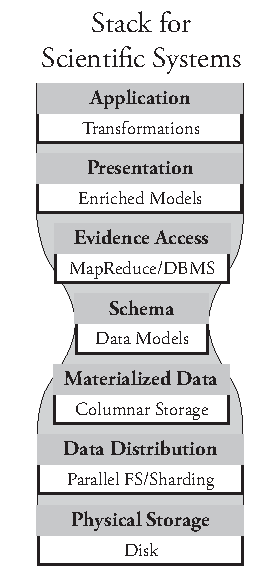
\includegraphics[width=0.6\linewidth]{stack-model.pdf}
\end{center}
\caption{A Stack Model for Scientific Analysis}
\label{fig:stack-model}
\end{figure}

Specifically, we need to:

\begin{enumerate}
\item Show how current systems fit into the stack model, and how our proposed stack is different
\item Elucidate why it is more efficient to build systems that are decomposed as per our stack above
(reference networking stack and protocol interchange), see Bafna et al~\cite{bafna13}, talk about costs
of programming without good stack model
\end{enumerate}

\subsection{Execution Platforms}
\label{sec:execution-platforms}

\textbf{TL;DW}; need to have a good discussion of what applications are good for MapReduce, what
are good on top of a database, what are good on an HPC farm, what should be done with an
abacus, etc. Needs to be written carefully to show the virtues of the Figure~\ref{fig:stack-model}
stack, while being frank about weaknesses.

\section{Implementation}
\label{sec:implementation}

\subsection{Genomics Pipeline}
\label{sec:genomics-pipeline}

Compare/contrast to current pipelines; talk about what the stages do in reasonable but not
excessive detail. Make reference to WHAM~\cite{li11} to show that this is an application domain that
SIGMOD has determined to be important.

\subsection{Coordinate System Joins}
\label{sec:coordinate-system-joins}

This will be a compare/contrast discussion of the multiple join algorithms we've created. TBD.

\subsection{Loading Remote Data}
\label{sec:loading-remote-data}

\begin{enumerate}
\item Data may not be kept locally
\begin{enumerate}
\item Too much data to keep locally
\item Not all data is hot
\end{enumerate}
\item May push data off local disks into block store
\item Manually re-staging data has high latency cost $\rightarrow$ impacts throughput
\item What do we need to do to accommodate this?
\begin{enumerate}
\item Efficient indexing
\item Remote push-down predicate
\end{enumerate}
\item Discuss S3/Parquet interaction
\end{enumerate}

\section{Performance}
\label{sec:performance}

This section will address:

\begin{itemize}
\item Performance of ADAM on real datasets
\item Compression achieved by Parquet
\item Examples extending the proposed stack to Astronomy
\end{itemize}

Experiments to run:

\begin{itemize}
\item General demonstration of scaling for genomics pipeline; updated experiments from TR
\item Experiments on coordinate system joins; broadcast vs. partition join strategies
\item Experiments showing benefit from performing remote data access without staging
\end{itemize}

\section{Discussion}
\label{sec:discussion}

\subsection{Scientific Processing on MapReduce}
\label{sec:scientific-compute-mr}

Big critique from SciDB camp is that MR is an inappropriate platform for scientific computing due to
lack of support for linear algebra. We need to counter this point, by allusion to performance on
algorithms above, and by alluding to specialized libraries for ML \& graph processing~\cite{sparks13,
xin13}.

Also, note that we don't argue that MR is the correct platform for particle simulations and other
traditional MPI workloads. However, MPI is the \emph{wrong} platform for most analyses.

Also, note that most scientific workloads require applying a UDF across a large set of data. This is not
inefficient to \emph{run} on a database, but it is inefficient to \emph{write}; SQL is a poor language for
scientific/statistical computing.

\subsection{Cost of Non-Commodity Systems}
\label{sec:commodity}

The advantage of the stack model we propose is that it enables the use and reuse of commodity
systems, instead of re-inventing the wheel (or, inventing a \emph{slightly} different wheel).

\section{Conclusion}
\label{sec:conclusion}

In the end, we conclude.

\appendix

\bibliographystyle{abbrv}
\bibliography{adam} 

%\balancecolumns
% That's all folks!
\end{document}
